% !TeX program = pdflatex
\documentclass[aspectratio=169,11pt]{beamer}

\usetheme{Madrid}
\usecolortheme{default}
\usefonttheme{professionalfonts}
\setbeamercovered{transparent}

\setbeamertemplate{footline}{%
  \hfill\insertframenumber\,/\,\inserttotalframenumber\hspace{2mm}\vspace{2mm}%
}
\setbeamertemplate{navigation symbols}{}

\usepackage{amsmath,amssymb,mathtools,mathrsfs,bm,array}
\usepackage{bbm}
\usepackage{tikz}
\usetikzlibrary{arrows.meta,positioning,calc}
\usepackage{hyperref}

\definecolor{feiblue}{RGB}{22,78,128}
\definecolor{feigreen}{RGB}{45,110,62}
\definecolor{feired}{RGB}{145,48,48}
\definecolor{feilight}{RGB}{245,247,250}

\setbeamercolor{titlelike}{fg=white}
\setbeamercolor{frametitle}{fg=white,bg=feiblue}
\setbeamercolor{block title}{fg=white,bg=feiblue}
\setbeamercolor{block body}{fg=black,bg=feilight}
\setbeamercolor{alertblock title}{fg=white,bg=feired}
\setbeamercolor{alertblock body}{fg=black,bg=red!5}
\setbeamercolor{exampleblock title}{fg=white,bg=feigreen}
\setbeamercolor{exampleblock body}{fg=black,bg=green!5}

\AtBeginSection[]{
\begin{frame}[plain]
  \vfill
  \begin{center}
    {\usebeamerfont{title}\color{feiblue}\insertsectionhead}
  \end{center}
  \vfill
\end{frame}
}

\newcommand{\R}{\mathbb{R}}
\newcommand{\E}{\mathbb{E}}
\newcommand{\cP}{\mathcal{P}}
\newcommand{\dd}{\,\mathrm{d}}
\newcommand{\one}{\mathbbm{1}}
\newcommand{\abs}[1]{\left\lvert#1\right\rvert}
\newcommand{\norm}[1]{\left\lVert#1\right\rVert}
\newcommand{\ip}[2]{\left\langle#1,#2\right\rangle}
\newcommand{\blue}[1]{{\color{blue}#1}}
\newcommand{\onslidecite}[1]{\par\vspace{0.4ex}\hfill{\scriptsize\color{black!60}#1}}
\DeclareMathOperator{\Att}{Att}

\title{Self-Attention as an Interacting Particle System}
\subtitle{Exact finite-token identities, regularity, and marked particles}
\author{Fei Lu}
\date{Fall 2026}

\begin{document}

%======================================================================
\begin{frame}
  \titlepage
\end{frame}

%----------------------------------------------------------------------
\begin{frame}{The Mathematical Question}
For tokens $x_1,\ldots,x_N\in\R^d$, one attention head forms
\[
  x_i^+=x_i+h\sum_{j=1}^N a_{ij}(X)Vx_j,
  \qquad
  a_{ij}(X)=
  \frac{e^{\ip{Qx_i}{Kx_j}/\tau}}
       {\sum_{r=1}^Ne^{\ip{Qx_i}{Kx_r}/\tau}}.
\]

\begin{block}{Questions for this section}
\begin{enumerate}
\item In what precise sense is this an interacting particle system?
\item What is exact at finite $N$, and what requires a mean-field limit?
\item Which regularity assumptions make the dynamics stable?
\item How do positions, masks, multiple heads, and local maps enter?
\end{enumerate}
\end{block}
\end{frame}

%----------------------------------------------------------------------
\begin{frame}{Outline of the Section}
\begin{columns}[T,onlytextwidth]
\column{0.48\textwidth}
\begin{block}{I. Exact particle structure}
\begin{itemize}
\item one-head empirical-measure identity;
\item nonlinear pushforward;
\item permutation equivariance;
\item exchangeability;
\item alternative spherical and linear fields.
\end{itemize}
\end{block}

\column{0.48\textwidth}
\begin{exampleblock}{II. Analysis and architecture}
\begin{itemize}
\item query and measure regularity;
\item the role of temperature;
\item marked measures and causal masks;
\item multi-head attention and token-wise maps;
\item forward questions: depth, clustering, learning.
\end{itemize}
\end{exampleblock}
\end{columns}
\end{frame}

%======================================================================
\section{The Exact Empirical-Measure Representation}

%----------------------------------------------------------------------
\begin{frame}{One Head: Scores, Weights, and Values}
Let
\[
 q_i=Qx_i,\qquad k_j=Kx_j,\qquad v_j=Vx_j,
\]
where $Q,K\in\R^{d_k\times d}$ and $V\in\R^{d_v\times d}$.  Define
\[
 s_\theta(x,y)=\frac{\ip{Qx}{Ky}}{\tau},
 \qquad
 a_{ij}(X)=\frac{e^{s_\theta(x_i,x_j)}}
                  {\sum_{r=1}^N e^{s_\theta(x_i,x_r)}}.
\]

\begin{itemize}
\item $x_i$ is the query particle; all $x_j$ are candidate key--value particles.
\item Each row $(a_{i1},\ldots,a_{iN})$ is a probability vector.
\item The usual scaling $\tau=\sqrt{d_k}$ prevents dot products from growing with $d_k$ under an isotropic heuristic.
\end{itemize}

\begin{alertblock}{First warning}
Row stochasticity is normalization, not a physical conservation law.
\end{alertblock}
\end{frame}


%----------------------------------------------------------------------
\begin{frame}{Empirical Measure form of Attention}
For $\mu\in\cP(\R^d)$ and  $\mu^N=\frac1N\sum_{j=1}^N\delta_{x_j}$, define
\[
 Z_\theta[\mu](x)
 =\int e^{s_\theta(x,y)}\,\mu(\dd y),
\quad  
 \Phi_\theta[\mu](x)
 =\frac{\displaystyle\int e^{s_\theta(x,y)}Vy\,\mu(\dd y)}
        {\displaystyle\int e^{s_\theta(x,y)}\,\mu(\dd y)}.
\]
\[ 
 Z_\theta[\mu^N](x)=\frac1N\sum_{j=1}^N e^{s_\theta(x,x_j)},
\quad 
 \Phi_\theta[\mu^N](x_i)
 =\frac{N^{-1}\sum_j e^{s_\theta(x_i,x_j)}Vx_j}
        {N^{-1}\sum_r e^{s_\theta(x_i,x_r)}}
 =\sum_{j=1}^N a_{ij}(X)Vx_j.
\]

\begin{itemize}
  \item  
For a fixed query $x$, attention first tilts $\mu$ by the score:
\[
 \pi_x^\mu(\dd y)
 =\frac{e^{s_\theta(x,y)}}{Z_\theta[\mu](x)}\,\mu(\dd y),
 \qquad
 \Phi_\theta[\mu](x)=\int Vy\,\pi_x^\mu(\dd y).
\]
\item A deterministic identity. No approximation or limit is needed. 
\end{itemize}
\end{frame}




%----------------------------------------------------------------------
\begin{frame}{Attention Is Not a Fixed Pair Kernel}
A classical mean-field interaction has (linear in $\mu$)
\[
 b[\mu](x)=\int b(x,y)\,\mu(\dd y).
\]
Attention instead has the effective kernel (nonlinear in $\mu$)
\[
 b_\mu(x,y)
 =\frac{e^{s_\theta(x,y)}Vy}{Z_\theta[\mu](x)},
 \qquad
 \Phi_\theta[\mu](x)=\int b_\mu(x,y)\,\mu(\dd y).
\]

\begin{block}{Structural difference}
The denominator couples every pair contribution to the entire token cloud.
Hence a theorem for a fixed Lipschitz pair kernel $b(x,y)$ does not apply verbatim; one must estimate $\Phi_\theta$ directly in both $x$ and $\mu$.
\end{block}
\end{frame}

%----------------------------------------------------------------------
\begin{frame}{Row Stochasticity Is Not a Conservation Law}
For the consensus-style dynamics
\[
 \dot x_i=\sum_j a_{ij}(X)(x_j-x_i),
\]
the empirical mean obeys
\[
 \frac{\dd}{\dd t}\frac1N\sum_i x_i
 =\frac1N\sum_j\left(\sum_i a_{ij}-1\right)x_j.
\]

\begin{itemize}
\item $\sum_j a_{ij}=1$: every row is stochastic.
\item Mean conservation additionally requires $\sum_i a_{ij}=1$: every column is stochastic.
\item Standard residual attention $\dot x_i=\sum_j a_{ij}Vx_j$ is not even in difference form.
\end{itemize}

\begin{alertblock}{Conclusion}
Momentum, energy, and token averages are not automatically conserved.  Such structure must be designed and proved.
\end{alertblock}
\end{frame}



%======================================================================
\section{Symmetry, Exchangeability, and Alternative Fields}

%----------------------------------------------------------------------
\begin{frame}{Column-Token Matrix Form of Attention}
With $X=(x_1,\ldots,x_N)\in\R^{d\times N}$,
\[
 S(X)=\frac1\tau X^\top Q^\top KX,
 \qquad A(X)=\operatorname{softmax}_{\rm row}(S(X)).
\]
If $d_v=d$, then
\[
  \Att(X)=VXA(X)^\top,
  \qquad X^+=X+h\Att(X).
\]

\begin{block}{Check the $i$th column}
\[
 [VXA^\top]_{:i}=\sum_{j=1}^N Vx_j A_{ij}
 =\sum_{j=1}^N a_{ij}(X)Vx_j.
\]
\end{block}

If $d_v\neq d$, an output map $O:\R^{d_v}\to\R^d$ is inserted before the residual addition.
\end{frame}


%----------------------------------------------------------------------
\begin{frame}{Permutation Equivariance}
Let $P\in\R^{N\times N}$ be a permutation matrix.  Without positions or masks,
\[
 \boxed{\Att(XP)=\Att(X)P.}
\]

\begin{proof}[Proof in three identities]
\begin{align*}
 S(XP)&=P^\top S(X)P,\\
 A(XP)&=P^\top A(X)P,\\
 \Att(XP)&=VXP\,A(XP)^\top
          =VXA(X)^\top P.
\end{align*}
The second identity holds because row-wise softmax commutes with simultaneous row and column relabeling.
\end{proof}

Equivariance does not say that all tokens have equal outputs.  It says that renaming the input tokens renames their outputs in the same way.
\end{frame}

%----------------------------------------------------------------------
\begin{frame}{Empirical Measure versus Exchangeability}
\small
\begin{block}{Deterministic statement}
For every tuple $(x_1,\ldots,x_N)$, the empirical measure $\mu^N$ exists and the attention identity holds.  No distributional assumption is needed.
\end{block}

\begin{exampleblock}{Probabilistic statement}
If $X$ is random and exchangeable, $XP\stackrel{d}=X$, then equivariance gives
\[
 \Att(X)P=\Att(XP)\stackrel{d}=\Att(X).
\]
Thus a content-only attention layer with shared parameters preserves exchangeability.
\end{exampleblock}

\begin{itemize}
\item Parameter sharing makes the unmarked empirical measure a closed state variable.
\item Exchangeability supports representative-particle and propagation-of-chaos arguments.
\item Exchangeability alone need not give a deterministic limit: the directing measure can be random.
\end{itemize}
\end{frame}

%----------------------------------------------------------------------
\begin{frame}{Which Architectural Changes Break the Unmarked Closure?}
\begin{center}
\begin{tabular}{p{0.28\textwidth}|p{0.30\textwidth}|p{0.31\textwidth}}
operation & unmarked empirical measure & remedy \\
\hline
shared $Q,K,V$ & closed & none \\
fixed position encodings & loses state--position pairing & position marks \\
causal mask & needs order and visibility & ordered marks and mask \\
token-specific parameters & index affects dynamics & parameter/type marks \\
dropout & random update not encoded & random marks or stochastic map
\end{tabular}
\end{center}


\end{frame}

%----------------------------------------------------------------------
\begin{frame}{Projected Identity Attention on the Sphere}
For $x\in\mathbb S^{d-1}$, let $P_x^\perp=I-xx^\top$.  Define
\[
 b_\gamma^{\rm sph}[\mu](x)
 =P_x^\perp
   \frac{\int e^{\gamma\ip{x}{y}}y\,\mu(\dd y)}
        {\int e^{\gamma\ip{x}{y}}\,\mu(\dd y)}.
\]

\begin{itemize}
\item At $\mu^N$, this is again an exact empirical-measure interaction.
\item Since $x^\top P_x^\perp=0$, the flow preserves $\abs{x}=1$.
\item Projection removes radial growth and exposes angular clustering.
\item The denominator still creates a state-dependent normalized kernel.
\end{itemize}

\onslidecite{Geshkovski--Letrouit--Polyanskiy--Rigollet (2023); Rigollet (2026)}
\end{frame}

%----------------------------------------------------------------------
\begin{frame}{Projected Linear Attention and an Oja-Type Flow}
\small
Let
\[
 M[\mu]=\int yy^\top\,\mu(\dd y),
 \qquad A=K^\top Q,
\]
and define
\[
 b_{A,V}^{\rm lin}[\mu](x)=P_x^\perp V M[\mu]Ax.
\]
At an empirical measure,
\[
 b_{A,V}^{\rm lin}[\mu^N](x_i)
 =P_{x_i}^\perp\frac1N\sum_j
   \ip{x_j}{Ax_i}Vx_j.
\]

\begin{exampleblock}{Oja special case}
If $A=V=I$ and $M$ is frozen, then
\[
 \dot x=P_x^\perp Mx
\]
is the spherical gradient-ascent flow of $\tfrac12 x^\top Mx$; stable directions select leading eigenspaces of $M$.
\end{exampleblock}

% \blue{Self-consistency makes $M=M[\mu_t]$ evolve, but in this matched identity case it does not destroy the gradient structure; the next slide identifies the energy.}
\end{frame}

%----------------------------------------------------------------------
\begin{frame}{A Useful Comparison}
\begin{center}
\scriptsize
\begin{tabular}{@{}p{0.22\textwidth}|p{0.20\textwidth}|p{0.21\textwidth}|p{0.22\textwidth}@{}}
model & interaction & geometry & main difficulty \\
\hline
fixed pair IPS & $\int b(x,y)\mu(\dd y)$ & Euclidean & singular or nonlinear $b$ \\
softmax attention & normalized exponential tilt & Euclidean & denominator and temperature \\
projected softmax & normalized tilt, then $P_x^\perp$ & sphere & clustering and metastability \\
projected linear & $P_x^\perp V M[\mu]Ax$ & sphere & evolving covariance, signs
\end{tabular}
\end{center}

\begin{block}{Common analytical route}
Identify $b[\mu](x)$, prove regularity in $x$ and $\mu$, control the state space, derive the measure equation, and only then study clustering or mean-field limits.
\end{block}
\end{frame}



%======================================================================
\section{Regularity of the Attention Field}


%----------------------------------------------------------------------
\begin{frame}{A Nonlinear Pushforward on Measures}
Set
\[
 T_{\theta,\mu}^h(x)=x+h\Phi_\theta[\mu](x).
\]
The token update is equivalent to the exact measure update
\[
 \boxed{
 \mu^{N,+}=\bigl(T_{\theta,\mu^N}^h\bigr)_\#\mu^N.}
\]

\begin{itemize}
  \item Nonlinear: 
For a fixed map $T$, the operation $\mu\mapsto T_\#\mu$ is linear in $\mu$.
Here the map $T_{\theta,\mu}^h$ itself depends on $\mu$, so
\[
 \mu\longmapsto\bigl(T_{\theta,\mu}^h\bigr)_\#\mu
\]
is generally nonlinear.
\end{itemize}
\end{frame}



%----------------------------------------------------------------------
\begin{frame}{Exact Identity, Mean Field, and Continuous Depth}
\begin{center}
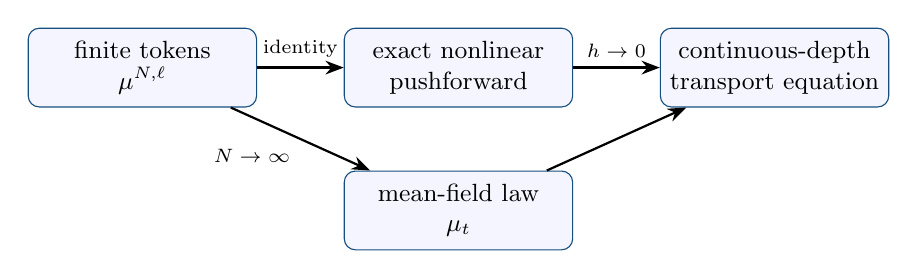
\begin{tikzpicture}[>=Stealth,node distance=8mm and 11mm,
  box/.style={draw=feiblue,rounded corners,fill=blue!4,align=center,
              minimum height=10mm,minimum width=29mm,font=\small}]
\node[box] (finite) {finite tokens\\$\mu^{N,\ell}$};
\node[box,right=of finite] (push) {exact nonlinear\\pushforward};
\node[box,right=of push] (depth) {continuous-depth\\transport equation};
\node[box,below=of push] (mf) {mean-field law\\$\mu_t$};
\draw[->,thick] (finite)--node[above,font=\scriptsize]{identity}(push);
\draw[->,thick] (push)--node[above,font=\scriptsize]{$h\to0$}(depth);
\draw[->,thick] (finite)--node[below left,font=\scriptsize]{$N\to\infty$}(mf);
\draw[->,thick] (mf)--(depth);
\end{tikzpicture}
\end{center}

\begin{alertblock}{Do not conflate the arrows}
\begin{itemize}
\item The empirical-measure formula is an algebraic identity.
\item $N\to\infty$ requires convergence of initial empirical laws and stability in the measure argument; probabilistic propagation of chaos needs more.
\item $h\to0$ requires a residual scaling and depth-regular parameters.
\end{itemize}
\end{alertblock}
\end{frame}


%----------------------------------------------------------------------
\begin{frame}{Why Bounded Support Appears}
For bilinear scores,
\[
 e^{s_\theta(x,y)}
 =\exp\!\left(\frac{\ip{Qx}{Ky}}{\tau}\right).
\]
Finite polynomial moments of $\mu$ do not by themselves control this exponential tilt.

If $x,y\in B_R$ and
\[
 \kappa=\frac{\norm Q\norm K}{\tau},
 \qquad S=\kappa R^2,
\]
then
\[
 e^{-S}\le e^{s_\theta(x,y)}\le e^S,
 \qquad
 e^{-S}\le Z_\theta[\mu](x)\le e^S.
\]

\begin{block}{Analytical payoff}
The normalizer is uniformly separated from zero, and both numerator and denominator have controlled Lipschitz constants.
\end{block}
\end{frame}

%----------------------------------------------------------------------
\begin{frame}{Query Sensitivity Is a Covariance}
Write $\pi_x^\mu$ for the tilted law.  Differentiating in $x$ gives
\[
 D_x\Phi_\theta[\mu](x)
 =\frac1\tau
 \operatorname{Cov}_{Y\sim\pi_x^\mu}
 \bigl(VY,\,Q^\top KY\bigr).
\]
On $B_R$,
\[
 \norm{D_x\Phi_\theta[\mu](x)}
 \le \norm V\frac{\norm Q\norm K}{\tau}R^2.
\]

\begin{exampleblock}{Interpretation}
When all highly attended values are nearly identical, the covariance is small even if the scores are sharp.  Sensitivity is largest near a competition between different keys.
\end{exampleblock}
\end{frame}

%----------------------------------------------------------------------
\begin{frame}{Measure Sensitivity: Control a Quotient}
Write
\[
 N_\mu(x)=\int e^{s_\theta(x,y)}Vy\,\mu(\dd y),
 \qquad
 Z_\mu(x)=\int e^{s_\theta(x,y)}\,\mu(\dd y).
\]
Then
\[
 \Phi[\mu](x)-\Phi[\nu](x)
 =\frac{N_\mu-N_\nu}{Z_\mu}
 +N_\nu\frac{Z_\nu-Z_\mu}{Z_\mu Z_\nu}.
\]

For measures supported in $B_R$, Kantorovich--Rubinstein duality gives
\[
 \abs{\mu(f)-\nu(f)}\le \operatorname{Lip}(f)W_1(\mu,\nu).
\]

\begin{alertblock}{Why the constant can be large}
Both inverse denominators cost factors of $e^S$; a small mass placed at a much higher-scoring key can be exponentially amplified.
\end{alertblock}
\end{frame}

%----------------------------------------------------------------------
\begin{frame}{Lipschitz Continuity on a Common Ball}
Let $\mu,\nu$ be supported in $B_R$ and $x,x'\in B_R$.  Set
\[
 L_x=\norm V\,\kappa R^2,
 \qquad
 L_\mu=\norm V e^{2S}(1+2S).
\]
Then
\[
 \boxed{
 \abs{\Phi_\theta[\mu](x)-\Phi_\theta[\nu](x')}
 \le L_x\abs{x-x'}+L_\mu W_1(\mu,\nu).}
\]
Also,
\[
 \abs{\Phi_\theta[\mu](x)}\le \norm V R.
\]

\begin{block}{Two distinct constants}
$L_x$ grows polynomially with the score scale $S$, while a uniform measure perturbation bound can require exponential dependence on $S$.
\end{block}
\end{frame}

%----------------------------------------------------------------------
\begin{frame}{Example: A Score Tie Controls Query Sensitivity}
Take $d=1$, $Q=K=V=1$, and
\[
 \mu=\tfrac12(\delta_{-R}+\delta_R).
\]
Then
\[
 \Phi[\mu](x)=R\tanh(Rx/\tau),
 \qquad
 \Phi'[\mu](x)=\frac{R^2}{\tau\cosh^2(Rx/\tau)}.
\]

\begin{itemize}
\item At $x=0$, the scores tie and $\Phi'[\mu](0)=R^2/\tau$.
\item Away from the tie, one key dominates and the derivative tends to zero.
\item Smaller temperature sharpens selection but worsens conditioning near ties.
\end{itemize}
\end{frame}

%----------------------------------------------------------------------
\begin{frame}{Example: Rare Preferred Mass Is Amplified}
Fix $x=R$, let $S=R^2/\tau$, and compare
\[
 \mu_0=\delta_{-R},
 \qquad
 \mu_\varepsilon=(1-\varepsilon)\delta_{-R}+\varepsilon\delta_R.
\]
The attention weight of $R$ is
\[
 p_\varepsilon
 =\frac{\varepsilon e^{2S}}
        {1-\varepsilon+\varepsilon e^{2S}}.
\]
Since $W_1(\mu_\varepsilon,\mu_0)=2R\varepsilon$,
\[
 \frac{\abs{\Phi[\mu_\varepsilon](R)-\Phi[\mu_0](R)}}
      {W_1(\mu_\varepsilon,\mu_0)}
 =\frac{e^{2S}}{1-\varepsilon+\varepsilon e^{2S}}
 \longrightarrow e^{2S}.
\]

The exponential measure-sensitivity factor is not merely a proof artifact.
\end{frame}

%----------------------------------------------------------------------
\begin{frame}{The Tokens Stay in a Common Ball on Finite Depth}
\small
For residual steps $h_\ell\ge0$, set
\[
 R_\ell=\max_i\abs{x_i^\ell}.
\]
The field bound gives
\[
 R_{\ell+1}
 \le (1+h_\ell\norm{V_\ell})R_\ell,
\]
and hence
\[
 R_\ell\le R_0
 \exp\!\left(\sum_{r<\ell}h_r\norm{V_r}\right).
\]
In continuous depth,
\[
 R(t)\le R_0\exp\!\left(\int_0^t\norm{V_s}\dd s\right).
\]

\begin{block}{Closing the argument}
Bounded initial tokens, bounded matrices, and temperature bounded away from zero give constants independent of $N$ on every finite depth interval.
\end{block}
\end{frame}

%----------------------------------------------------------------------
\begin{frame}{Temperature Is a Conditioning Parameter}
\begin{center}
\begin{tabular}{c|c|c}
regime & behavior & analytical cost \\
\hline
$\tau\downarrow0$ & nearly hard selection & large sensitivity near score ties \\
moderate $\tau$ & query-dependent averaging & balanced selectivity and stability \\
$\tau\uparrow\infty$ & nearly uniform weights & loss of query specificity
\end{tabular}
\end{center}

\begin{alertblock}{Tradeoff}
Sharper attention can increase expressivity at the same time that it worsens forward stability, mean-field approximation, and statistical robustness.
\end{alertblock}

This is a mathematical reason to track temperature explicitly rather than hide it in notation.
\end{frame}

%======================================================================
\section{Marked Particles and the Full Transformer Block}

%----------------------------------------------------------------------
\begin{frame}{Why the Unmarked Cloud Cannot Encode a Sequence}
The tuples
\[
 (x_1,x_2,x_3)
 \qquad\text{and}\qquad
 (x_3,x_1,x_2)
\]
have the same unmarked empirical measure.  A language model must nevertheless distinguish their orders.

Attach marks
\[
 z_i=(x_i,p_i,c_i),
 \qquad
 \nu^N=\frac1N\sum_i\delta_{z_i},
\]
where
\begin{itemize}
\item $p_i$ records position or time;
\item $c_i$ records role, modality, particle species, or other type information.
\end{itemize}

The empirical measure now forgets only the arbitrary list order, not the state--position pairing.
\end{frame}

%----------------------------------------------------------------------
\begin{frame}{Attention on a Marked State Space}
Let $z=(x,p,c)$ and $z'=(y,p',c')$.  Allow a score $s_\theta(z,z')$, a value $V_\theta(z')$, and a mask $m(p,p')\in\{0,1\}$.  Then
\[
 \Phi_\theta[\nu](z)
 =\frac{\int m(p,p')e^{s_\theta(z,z')}V_\theta(z')\,\nu(\dd z')}
        {\int m(p,p')e^{s_\theta(z,z')}\,\nu(\dd z')}.
\]
The exact marked update is
\[
 \nu^{N,+}=(\mathcal T_{\theta,\nu^N}^h)_\#\nu^N,
 \qquad
 \mathcal T_{\theta,\nu}^h(x,p,c)
 =(x+h\Phi_\theta[\nu](x,p,c),p,c).
\]

The marks remain fixed while the feature state evolves.
\end{frame}

%----------------------------------------------------------------------
\begin{frame}{Causal Attention Is a Marked Interaction}
For ordered positions, the causal mask is
\[
 m(p,p')=\one_{\{p'\le p\}}.
\]
At positions $p_i=i$, one row has weights
\[
 a_{ij}
 =\frac{\one_{\{j\le i\}}e^{s_{ij}}}
        {\sum_{r\le i}e^{s_{ir}}}.
\]

\begin{center}
\begin{tabular}{c|cccc}
 & $j=1$ & $j=2$ & $j=3$ & $j=4$\\
\hline
$i=1$ & $\checkmark$ & & &\\
$i=2$ & $\checkmark$ & $\checkmark$ & &\\
$i=3$ & $\checkmark$ & $\checkmark$ & $\checkmark$ &\\
$i=4$ & $\checkmark$ & $\checkmark$ & $\checkmark$ & $\checkmark$
\end{tabular}
\end{center}

Self-visibility makes the denominator positive for every empirical sequence, but the visible mass may be only $1/N$.
\end{frame}

%----------------------------------------------------------------------
\begin{frame}{A Hard Mask Can Destroy Wasserstein Continuity}
Take query position $p=1/2$, zero scores, and value $V(y,p')=y$.  Let
\[
 \nu=\tfrac12\delta_{(0,0)}+\tfrac12\delta_{(1,1/2)},
\]
\[
 \nu_\varepsilon
 =\tfrac12\delta_{(0,0)}+\tfrac12\delta_{(1,1/2+\varepsilon)}.
\]
Then
\[
 W_1(\nu_\varepsilon,\nu)\le\varepsilon/2\longrightarrow0.
\]
But the masked outputs are
\[
 \Phi[\nu](p)=\tfrac12,
 \qquad
 \Phi[\nu_\varepsilon](p)=0.
\]

\begin{alertblock}{Lesson}
A lower bound on visible mass controls division by the normalizer; it does not remove the discontinuity of a hard mask in a continuous position metric.
\end{alertblock}
\end{frame}

%----------------------------------------------------------------------
\begin{frame}{Multiple Heads Are a Sum of Interaction Fields}
For heads $m=1,\ldots,H$,
\[
 \Phi_{\boldsymbol\theta}[\mu](x)
 =\sum_{m=1}^H O_m
 \frac{\int e^{\ip{Q_mx}{K_my}/\tau_m}V_my\,\mu(\dd y)}
      {\int e^{\ip{Q_mx}{K_my}/\tau_m}\,\mu(\dd y)}.
\]

\begin{itemize}
\item $V_m:\R^d\to\R^{d_{v,m}}$ produces the head value.
\item $O_m:\R^{d_{v,m}}\to\R^d$ returns it to the residual stream.
\item Concatenation followed by $O=[O_1\ \cdots\ O_H]$ is exactly the displayed sum.
\item Different heads can probe different geometries, but the formula does not prevent redundancy.
\end{itemize}

\onslidecite{Vaswani et al. (2017)}
\end{frame}

%----------------------------------------------------------------------
\begin{frame}{The Rest of the Block Is Mostly Token-Wise}
A shared MLP has the form
\[
 f(x)=M_2\sigma(M_1x+b_1)+b_2.
\]
Layer normalization is a shared local map
\[
 \operatorname{LN}_{a,b,\varepsilon}(x)
 =a\odot\frac{x-\bar x\mathbf1}
 {\sqrt{d^{-1}\norm{x-\bar x\mathbf1}^2+\varepsilon}}+b.
\]

\begin{block}{Interaction versus local maps}
\begin{itemize}
\item Attention couples distinct tokens through $\mu^N$.
\item MLP and layer normalization act on one token at a time, with shared parameters.
\item A full block is therefore a composition of measure-dependent and local pushforwards.
\end{itemize}
\end{block}
\end{frame}

%----------------------------------------------------------------------
\begin{frame}{Exact Pre-Normalization Block}
Let $n_1,n_2$ be the two normalization maps.  Suppressing dropout,
\begin{align*}
 \eta&=(n_1)_\#\mu^N,\\
 y_i&=x_i+h\Phi_{\boldsymbol\theta}[\eta](n_1(x_i)),\\
 x_i^+&=y_i+h f(n_2(y_i)).
\end{align*}
Define
\[
 T_\mu^h(x)=x+h\Phi_{\boldsymbol\theta}[(n_1)_\#\mu](n_1(x)),
 \qquad
 G^h(y)=y+h f(n_2(y)).
\]
Then
\[
 \boxed{\mu^{N,+}=(G^h\circ T_{\mu^N}^h)_\#\mu^N.}
\]

This is an exact finite-depth representation of the deterministic block.
\end{frame}

%----------------------------------------------------------------------
\begin{frame}{When Can We Add the Two Vector Fields?}
Write
\[
 A_\mu(x)=\Phi_{\boldsymbol\theta}[(n_1)_\#\mu](n_1(x)),
 \qquad b=f\circ n_2.
\]
The exact composition is
\[
 G^h(T_\mu^h(x))=x+hA_\mu(x)+h b(x+hA_\mu(x)).
\]
If $b$ is $L_b$-Lipschitz and $\abs{A_\mu(x)}\le B$, then
\[
 \abs{G^h(T_\mu^h(x))-\bigl(x+h[A_\mu(x)+b(x)]\bigr)}
 \le h^2L_bB.
\]

\begin{block}{Interpretation}
The sum of the interaction and local fields is a first-order continuous-depth model.  It is not the exact block when $h=1$.
\end{block}
\end{frame}

%----------------------------------------------------------------------
\begin{frame}{What Else Must Be Modeled?}
\begin{itemize}
\item \textbf{Post-normalization:} changes the composition order.
\item \textbf{Gates:} $x^+=x+g(x)\odot F(x)$ change the local vector field.
\item \textbf{Dropout:} $D_\rho(u)=\xi\odot u/(1-\rho)$ introduces explicit randomness.
\item \textbf{Parameter variation with depth:} produces a nonautonomous particle system.
\item \textbf{Output/readout tokens:} may require additional types or distinguished marks.
\end{itemize}

\begin{alertblock}{Model before taking a limit}
Normalization order, masks, gates, and randomness determine the actual finite-layer map and therefore the assumptions needed for stability or continuous depth.
\end{alertblock}
\end{frame}

%======================================================================
\section{Synthesis and Problems}

%----------------------------------------------------------------------
\begin{frame}{The Section in One Diagram}
\begin{center}
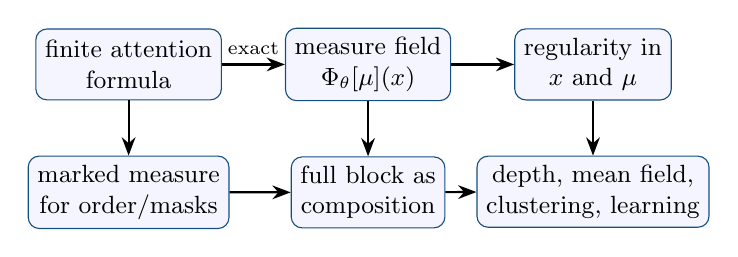
\begin{tikzpicture}[>=Stealth,node distance=7mm and 8mm,
  box/.style={draw=feiblue,rounded corners,fill=blue!4,align=center,
              minimum height=9mm,font=\small}]
\node[box] (formula) {finite attention\\formula};
\node[box,right=of formula] (measure) {measure field\\$\Phi_\theta[\mu](x)$};
\node[box,right=of measure] (regular) {regularity in\\$x$ and $\mu$};
\node[box,below=of formula] (marks) {marked measure\\for order/masks};
\node[box,below=of measure] (block) {full block as\\composition};
\node[box,below=of regular] (forward) {depth, mean field,\\clustering, learning};
\draw[->,thick] (formula)--node[above,font=\scriptsize]{exact}(measure);
\draw[->,thick] (measure)--(regular);
\draw[->,thick] (formula)--(marks);
\draw[->,thick] (marks)--(block);
\draw[->,thick] (measure)--(block);
\draw[->,thick] (regular)--(forward);
\draw[->,thick] (block)--(forward);
\end{tikzpicture}
\end{center}

\begin{block}{Central conclusion}
Self-attention is exactly a normalized, measure-dependent interaction at finite token number.  The IPS viewpoint becomes analytical only after the state, marks, scaling, and regularity regime are specified.
\end{block}
\end{frame}

%----------------------------------------------------------------------
\begin{frame}{Questions to Work Through}
\begin{enumerate}
\item Derive the covariance formula for $D_x\Phi_\theta[\mu](x)$.
\item Prove permutation equivariance from the matrix score formula.
\item Find a condition on $Q,K,V$ under which the unnormalized linear field is the gradient of an energy on the sphere.
\end{enumerate}

\begin{exampleblock}{Research question}
Which architectural constraint yields a useful compromise among expressivity, clustering, and a depth-uniform stability modulus?
\end{exampleblock}
\end{frame}

%----------------------------------------------------------------------
\begin{frame}{Selected References}
\small
\begin{itemize}
\item D.~Bahdanau, K.~Cho, and Y.~Bengio, ``Neural machine translation by jointly learning to align and translate,'' ICLR, 2015.
\item A.~Vaswani et al., ``Attention is all you need,'' NeurIPS, 2017.
\item B.~Geshkovski, C.~Letrouit, Y.~Polyanskiy, and P.~Rigollet, ``The emergence of clusters in self-attention dynamics,'' NeurIPS, 2023.
\item N.~Karagodin, Y.~Polyanskiy, and P.~Rigollet, ``Clustering in causal attention masking,'' NeurIPS, 2024.
\item P.~Rigollet, ``The mean-field dynamics of Transformers,'' ICM Proceedings, 2026.
\item \blue{M.~E. Sander, P.~Ablin, M.~Blondel, and G.~Peyr\'e,
``Sinkformers: Transformers with doubly stochastic attention,'' AISTATS, 2022.}
\item \blue{M.~Burger, S.~Kabri, Y.~Korolev, T.~Roith, and L.~Weigand,
``Analysis of mean-field models arising from self-attention dynamics in
Transformer architectures with layer normalization,'' Phil. Trans. R. Soc. A,
2025.}
% \item S.~Li et al., ``On the diverse dynamical behaviors arising in deep linear Transformers,'' 2026.
\end{itemize}

\vspace{1ex}
The full citations and the detailed proofs appear in the companion lecture notes.
\end{frame}


% %----------------------------------------------------------------------
% \begin{frame}{Gradient flow in Matched Symmetric Cases}
% \small
% \blue{For the identity Oja field on $\mathbb S^{d-1}$,
% \[
%  M[\mu]=\int yy^\top\,\mu(\dd y),
%  \qquad
%  \mathcal J_{\rm Oja}(\mu)
%  =\frac14\norm{M[\mu]}_F^2
%  =\frac14\iint\ip{x}{y}^2\,\mu(\dd x)\mu(\dd y).
% \]
% Its first variation satisfies
% \[
%  \nabla_{\mathbb S}\frac{\delta\mathcal J_{\rm Oja}}{\delta\mu}(x)
%  =P_x^\perp M[\mu]x=b_{I,I}^{\rm lin}[\mu](x).
% \]
% Thus the self-consistent Oja dynamics are the spherical $W_2$ gradient
% \emph{ascent} of $\mathcal J_{\rm Oja}$, or descent of
% $-\mathcal J_{\rm Oja}$.}

% \blue{The same mechanism applies to unnormalized projected identity-softmax.
% Set
% \[
%  Z_\mu(x)=\int e^{\gamma\ip{x}{y}}\,\mu(\dd y),\qquad
%  \mathcal J_\gamma(\mu)=\frac1{2\gamma}
%  \iint\bigl(e^{\gamma\ip{x}{y}}-1\bigr)\,\mu(\dd x)\mu(\dd y).
% \]
% Symmetry of the score gives
% \[
%  \nabla_{\mathbb S}\frac{\delta\mathcal J_\gamma}{\delta\mu}(x)
%  =P_x^\perp\int e^{\gamma\ip{x}{y}}y\,\mu(\dd y)
%  =:\widetilde b_\gamma[\mu](x),
% \]
% so $\partial_t\mu+\operatorname{div}_{\mathbb S}
% (\mu\widetilde b_\gamma[\mu])=0$ is again an ordinary spherical $W_2$
% gradient ascent.}
% \end{frame}

% %----------------------------------------------------------------------
% \begin{frame}{Softmax Changes the Metric}
% \small
% \blue{Row normalization divides the preceding gradient by its partition
% function:
% \[
%  b_\gamma[\mu](x)
%  =\frac{1}{Z_\mu(x)}
%  \nabla_{\mathbb S}\frac{\delta\mathcal J_\gamma}{\delta\mu}(x).
% \]
% Consequently, along a smooth solution,
% \[
%  \frac{\dd}{\dd t}\mathcal J_\gamma(\mu_t)
%  =\int_{\mathbb S^{d-1}}\frac1{Z_{\mu_t}(x)}
%  \left|\nabla_{\mathbb S}
%  \frac{\delta\mathcal J_\gamma}{\delta\mu}(x)\right|^2
%  \mu_t(\dd x)\geq0.
% \]
% This is a generalized gradient ascent with kinetic norm
% \[
%  \norm{v}_{\mu,m}^2
%  =\int_{\mathbb S^{d-1}} Z_\mu(x)|v(x)|^2\,\mu(\dd x),
% \]
% not the standard $W_2$ norm $\int|v|^2\dd\mu$.  The metric is therefore part
% of the statement ``attention is a gradient flow.''}
% \end{frame}

% %----------------------------------------------------------------------
% \begin{frame}{When Does the Structure Survive?}
% \small
% \begin{itemize}
% \item \blue{Burger et al.: if $D=Q^\top K=D^\top$ and $V=\pm D$, normalized
% spherical attention is a rigorous gradient flow for a modified transport
% metric.}
% \item \blue{Sander et al.: under their symmetry and sign compatibility,
% Sinkhorn-normalized attention is a standard $W_2$ gradient flow.}
% \item \blue{Generic $Q,K,V$, causal masks, or untied depth-dependent parameters
% need not admit one global energy; they retain the transport description.}
% \end{itemize}
% \blue{\textbf{Two different meanings of ``flow.''}  The statement above concerns
% the evolution of tokens, or of their law, with network depth as time.  It is
% not gradient descent of the training loss in parameter space.

% Moreover, a finite residual attention layer is a forward-Euler step of the
% depth-continuous flow.  Even when the limiting ODE is variational, a discrete
% layer decreases the energy only under an appropriate step-size condition.}

% \onslidecite{Sander--Ablin--Blondel--Peyr\'e (2022); Burger--Kabri--Korolev--Roith--Weigand (2025)}
% \end{frame}



\end{document}
